\section{Implementation and Methodologies}

This project had two major implementations, the annotator and the ML model,
which will be detailed in this chapter. The following will explain used
methodologies and choices made in the implementation process as well as overcome
difficulties. 

\subsection{Image-Annotator}

The purpose of the image annotation software is to give an easy possibility of
labeling, rescaling, cropping and saving images in order to be used as a dataset
by the ML model.
\newline
The software was completely written in python, an interpreted script language.
Still python has object oriented features, that where partly used in this
project. 
\newline
The program is structured in a way, to have two different classes,
"Window" and "popupWindow" to take care of the UI part of the project. The rest
of the functionality is structured into script-like functions. This structuring
makes it easier to split the program into smaller tasks that can be distributed
and worked on individually. This is a methodology oriented at the MVC (Model
View Controller) software development pattern. The UI is here clearly separated
from the controlling instance, that handles the backend of user interaction as
well as the model, which is responsible for data storage and maintenance. As
this is a simple single instance application, of course a detailed
implementation was not necessary and the model and controller are somewhat mixed
and both just represented as the separate functions. Still it gives the
possibility of separating the implementation of the UI, the backend and the
storage system.
\newline
The UI is handled by the the tkinter python library, which gives a lot of basic
functionality to easily implement the frontend of the application. The UI of
this project was mainly focused on the menu bar on top in addition to a
right-click menu. This choice was made in order to keep the overall frame clean
and focused on the most important thing, the image.
\newline
The backend storage uses a python dictionary to be able to store the edits at all times.
If need be, the entirety of the data can be saved to file using
the JSON format and loaded back from it as well. To keep the storage as
efficient as possible and maintain the possibility to easily change categories,
they are saved separately with a second array only linking the index of
the annotation to the index of a category. Listing 1 shows a reduced example of
stored annotations. There is a feature enabling the user to save every processed
resized image to a specified location. It was disabled as it turned out not to
be needed in this project. 

\begin{figure*}[t]
    \centering
    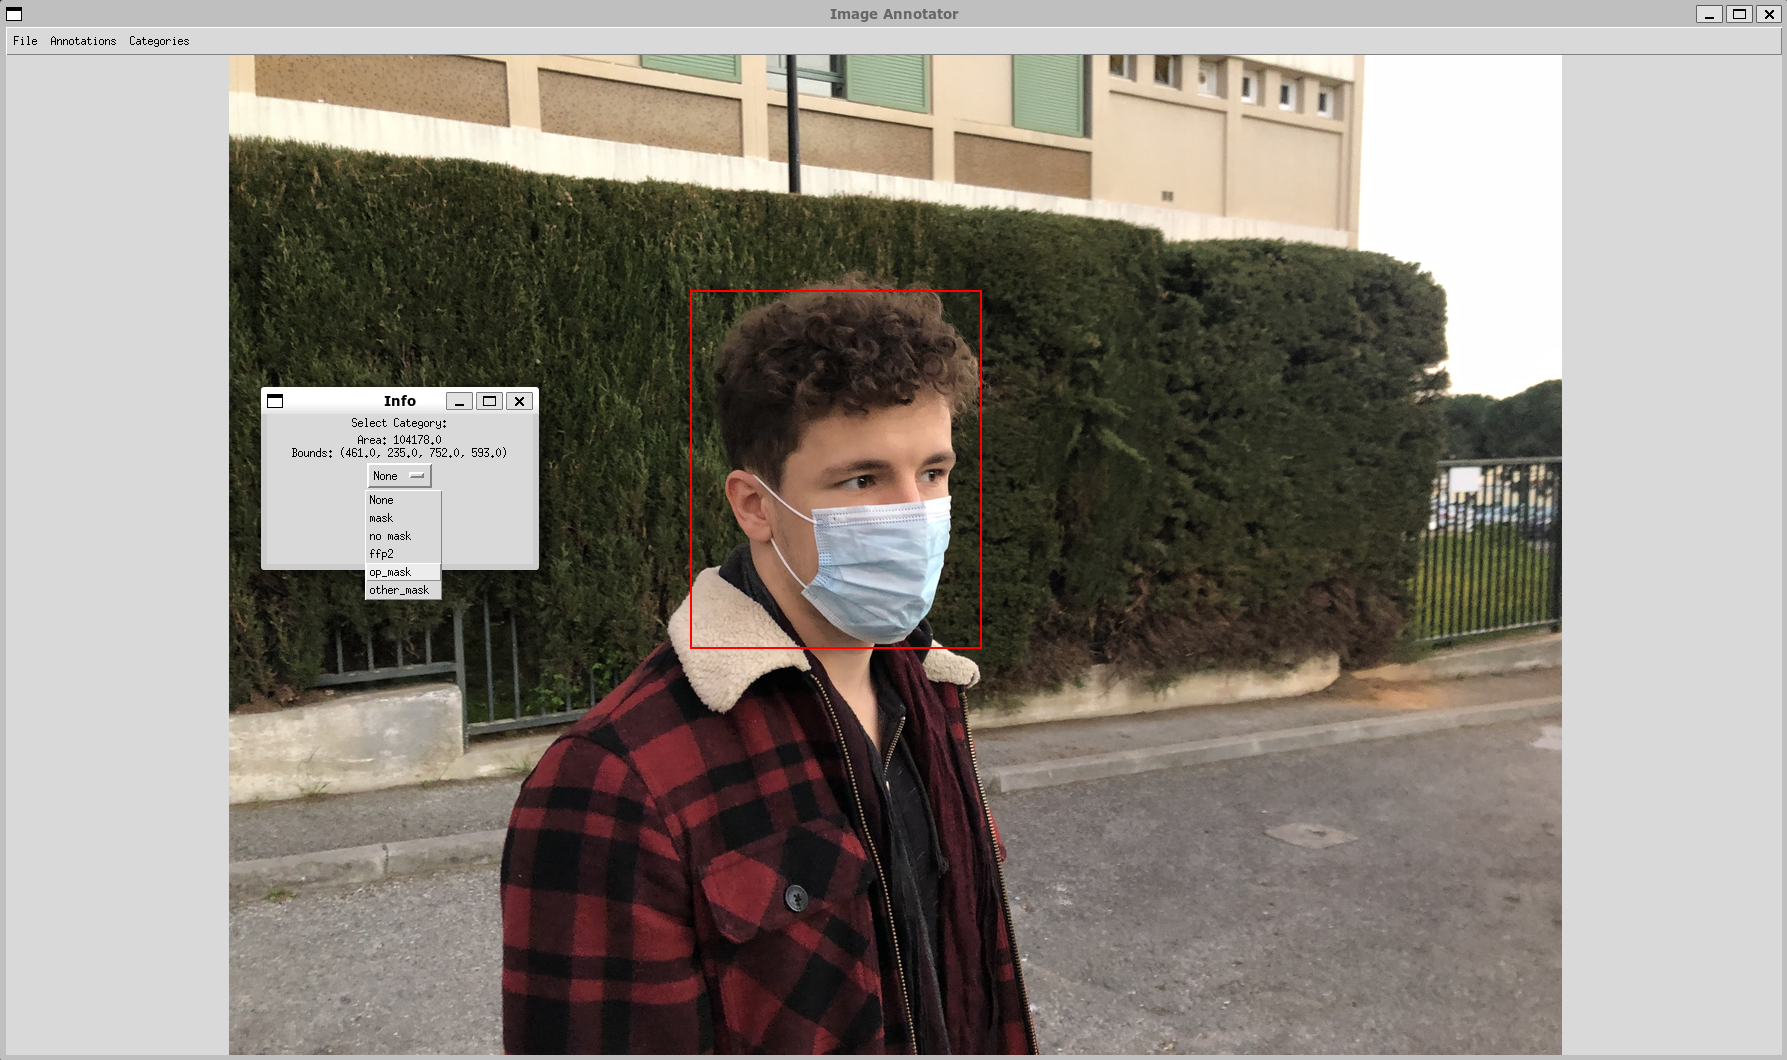
\includegraphics[width=\textwidth]{annotator_in_action.png}
    \caption{image annotator in action}
    \label{fig:anno}
\end{figure*}
\lstinputlisting[language=json,firstnumber=1,breaklines,caption={reduced example of saved annotations},captionpos=b, numbers=right]{../code/annotations.json}
The helping features are implemented as functions, that can be called through
the given menus:

\begin{description}[font=\sffamily\bfseries, leftmargin=1cm, style=nextline]
    \item[open image]
        Opens a file selector to let you chose an image to annotate
    \item[load next image]
        Finds the next image after natural order (the windows file-name order) in
        the same folder as the currently loaded image
    \item[save/import/view annotations]
        Lets the user chose a file location to either import or export all
        annotations as well as gives the possibility of viewing all currently
        loaded annotations in a list-view
    \item[add/replace/show category]
         Lets the user add a new category, replace an existing one or show all
         current categories in a list
    \item[import/export categories]
        Similar to annotations this gives the possibility to only share the
        categories by enabling exporting to json, csv or xlsx and importing from
        json and csv
    \item[replace/change destination]
        A feature that was not used during this project enabling the user to
        save each image resized and as png but not cropped to a specified
        location, that can be different for each image
\end{description}

Finally the main features of the annotation all lay in the mouse listeners. 
The user is able to draw rectangles in case an image was loaded.
A rectangle is only allowed if it has an area greater that 40 pixels, sides
longer than 5 pixels and is not overlapping with another rectangle by more than
20\%. If a valid rectangle is drawn, the user gets pointed details and can
chose a label. Figure \ref{fig:anno} shows the annotator in action. By
double-clicking or right-clicking the rectangle, this popup can be shown again
at any time and the label changed. Right-clicking also gives the choice of
deleting the rectangle.
\newline
This gives the annotator the needed functionality and enables a quick and
easy labeling of all the images. Once the labeling is done, the menu item
"\textbf{crop and save}" reloads each image at a time, crops all made rectangles
to 240x240 square format and saves them in folders according to their labeling
in a location specified by the user.

\subsection{Machine Learning Model}

The Classifier is also coded in python, using the tensorflow library,
specifically the keras API, which is one of the most used deep learning
frameworks. In addition the OpenCV library is used again for face recognition. 
\newline
The overall structure on this part of the project is based on the tensorflow
tutorials \cite{tut}. It is split up into loading and structuring the dataset,
pre-processing the images, then training the model and finally evaluating it's
effectiveness. In addition to that the code offers interfaces for using the
model to classify any kind of image, or even live-feed through a camera.
\newline
The first part of any machine learning algorithm is the dataset. It is used,
to train the network, by giving it an image to predict and improve its decision 
process through backpropagation, based on the answer. After
training, or even during the training process the dataset can be used to
determine the accuracy of the prediction. In order for this evaluation not to be
biased, the dataset has to be split into a train and a test or validation set:
\lstinputlisting[
    language=json,
    breaklines,
    caption={splitting the dataset},
    captionpos=b
    ]{../code/dataset.py}
This way the training can be done on separate data than the final validation of
the effectiveness of the model. Otherwise it could be, that the model can
specifically classify the images it trained on, but nothing else.
\newline
Next come the pre-processing. Especially with smaller datasets like the one used
here, it makes sense to gain a little more data by augmenting the images and
creating multiple different ones from one. This is done by random rotations,
shifts, flips and sometimes even change of contrast or similar features (Listing
3, line 1-9). The code used here was supported by the examples on the keras
documentation page \cite{zoom_range=0.2}.
\newline
A ML model has also problems with non-binary categorizations, which is why so
called one hot encoding on the labels can be helpful or even necessary (Listing
3, line 11,12). 
\newline
A common pre-processing step with images, is also the rescaling of color-values.
Usually they are saved as integer from 0 to 255. For a neural network it can be
easier to work with values between 0 and 1, which is why they can be rescaled by
multiplying each value with 1/255 (Listing 3, line 2).

\lstinputlisting[
    language=json,
    firstnumber=1,
    breaklines,
    caption={data augmentation and one hot encoding},
    captionpos=b
    ]{../code/preprocessing.py}

Now finally it is time for the model creation, compilation and training or
fitting. In the keras framework it is pretty simple to set up the layers one
wants to use in the network by simply adding them in order to the model. This
step is crucial, as it creates the overall network structure and determines how
good the model can be trained later. 
\newline
The model was inspired by multiple sources and refined by trial and error
\cite{Prakash2020}. \lstinputlisting[ language=json, firstnumber=1, breaklines,
caption={model layer structure}, captionpos=b, numbers=right ]{../code/model.py}
It uses alternating layers of convolution and max-pooling. This is the general
approach taken when doing an image classification. The convolution-layer uses a
filter to highlight certain features in the image, like edges for example, while
the max-pooling layers are responsible for summarizing pixels and therefore
simplifying the process. When going through training, the neural network will
adjust the filters used in the convolution-layers. Each convolution-layer has
the option relu (Rectified Linear Unit), which takes care, that all negative
values are turned into positive ones, so that the network doesn't get confused.
At the bottom there eventually is a flattening-layer as well as two
dense-layers. As the convolution-layers work with image-data, represented as
matrixes; they need to be flattened back to one dimension in order for the
network to make a decision. Finally the two dense-layers are condensing the
output down to exactly the number of classes we have so that the network is able
to gives us an answer. Before the the dense-layers we also added a
dropout-layer, that will already eliminate low confidences, so they won't mess
up any other information reaching that state.
\newline
After setting up the structure, the model can be compiled using an optimizer as
well as what should be optimized and finally fitted to the dataset. Especially
while the fitting process it is important to specify a good amount of training
epochs the model should go through, as using to few will leave potential unused
and using to many will take a lot of time, and not do any more good.
\lstinputlisting[
    language=json,
    firstnumber=1,
    breaklines,
    caption={model compilation and fitting},
    captionpos=b, 
    numbers=right
    ]{../code/compile_and_fit.py}
The loss-function we used, is the "mean\_squared\_error"-function as it performed
slightly better compared to the other loss-functions. More details on that
follow in the next chapter.
\newline
To make the model easier accessible, the functionality was added to the image
annotation software as well. It offers a new tab in the top menu bar with a few
functions:
\begin{description}[font=\sffamily\bfseries, leftmargin=1cm, style=nextline]
    \item[train model]
        this lets the user chose a directory which includes all labeled folders
        with the respective dataset images; using this directory it loads the
        dataset and trains the model; the output window unfortunately only shows
        the whole output in the end, so the user has to wait a while
    \item[save/load model]
        saves or loads the model in two separate files; one contains all keras
        settings needed to run the model, the other one, contains label names as
        well as necessary images sizes for the model to integrate into the
        annotator 
    \item[classify current image]
        this function takes all boxes drawn on the current window, that where
        labeled with "None", crops them, and lets the model decide the correct
        label; the label is set automatically and displayed on screen
    \item[live classification]
        this is an experimental feature, that opens the camera and for each
        shown frame, uses the OpenCV library to cut out faces and plugging them
        into the ML model; in the end it is able to tell on the live feed
        whether a person is wearing a mask or not
\end{description}
